\documentclass[11pt,a4paper]{article}
\usepackage{gtu-el-yazisi}
\begin{document}
\notbilgi{Analog Haberleşme}{Bozulmasız iletim, filtreler ve modülasyon}{Ders6.pdf}

\section{Bozulmasız iletim}
\sayfa{1}
(Distortionless Transmission)
\begin{center}
\begin{tikzpicture}[>=Stealth, line width=0.7pt]
  \node[draw, minimum width=1.8cm, minimum height=0.9cm] (h) at (0,0) {$h(t)$};
  \draw[->] (-2.4,0) -- (h.west);
  \node[above] at (-1.9,0) {$x(t)$};
  \draw[->] (h.east) -- (1.4,0);
  \node[right] at (1.4,0) {$y(t)=k\,x(t-t_d)$};
  \node[below] at (0,-0.5) {kanal};
\end{tikzpicture}
\end{center}
\begin{align*}
  y(t) &= K\cdot x(t-t_d) \\
  Y(f) &= k\,X(f)\,e^{-j2\pi f t_d} \\
  H(f) &= \frac{Y(f)}{X(f)} = k\,e^{-j2\pi f t_d} \\
  &= |H(f)|\,e^{j\theta_h(f)}
\end{align*}
\[
  \left\{\begin{aligned} |H(f)| &= |k|\ \checkmark \\ \theta_h(f) &= -2\pi f t_d\ \checkmark \end{aligned}\right.
  \qquad\qquad \mathcal{F}^{-1}\ \downarrow
\]
\[
  \textcolor{kirmizikalem}{\star}\ \kutula{h(t)=k\,\delta(t-t_d)}
\]

\noindent
\begin{minipage}[c]{0.46\linewidth}
  \centering
  Bozulmasız sistem\\[1mm]
  \begin{tikzpicture}[>=Stealth, line width=0.7pt, scale=0.9]
    \draw[->] (-2,0) -- (2,0);
    \draw[->] (0,0) -- (0,1.8) node[right] {$|H(f)|$};
    \draw (-1.8,1.0) -- (1.8,1.0);
    \node[above right] at (0,1.0) {$|k|$};
  \end{tikzpicture}
\end{minipage}\hfill
\begin{minipage}[c]{0.5\linewidth}
  \centering
  \begin{tikzpicture}[>=Stealth, line width=0.7pt, scale=0.9]
    \draw[->] (-2,0) -- (2,0) node[right] {$f$};
    \draw[->] (0,-1.6) -- (0,1.6) node[right] {$\theta_h(f)$};
    \draw (-1.5,1.2) -- (1.5,-1.2);
    \node[below right] at (1.2,-0.95) {$-2\pi f t_d$};
  \end{tikzpicture}
\end{minipage}
\begin{gather*}
  \text{Grup gecikmesi}=t_d(f)=-\frac{1}{2\pi}\,\frac{d\theta_h(f)}{df}\quad\text{(Group / envelope delay)} \\
  \theta_h(f)=2\pi f t_d\ \Rightarrow\ t_d(f)=\underset{\textcolor{kirmizikalem}{\star\ \text{sabit}}}{t_d}\footnotemark
\end{gather*}
\footnotetext{Claude notu: önceki satıra göre muhtemelen $\theta_h(f)=-2\pi f t_d$ olmalı.}

\begin{ornek}
  \begin{center}
  \begin{circuitikz}[line width=0.7pt]
    \draw (0,2) to[R=$\qty{1}{\kilo\ohm}$, o-*] (3.5,2) to[short, -o] (6.2,2);
    \draw (3.5,2) to[C, l={$C=10^{-9}\,\si{\farad}$}] (3.5,0);
    \draw (0,0) to[short, o-*] (3.5,0) to[short, -o] (6.2,0);
    \node[left] at (-0.1,2) {$+$};
    \node[left] at (-0.1,0) {$-$};
    \node[left] at (-0.3,1) {$x(t)$};
    \node[right] at (6.3,2) {$+$};
    \node[right] at (6.3,0) {$-$};
    \node[right] at (6.5,1) {$y(t)$};
  \end{circuitikz}
  \end{center}
  Bu filtreden işaretin bozulmadan geçmesi için $x(t)$'nin bant genişliği ne olmalıdır?
  (\%2'lik genlik cevabı toleransı, \%5'lik grup gecikmesi toleransı mevcuttur.)
\end{ornek}
Alçak geçiren filtre
\begin{align*}
  H(f)=\frac{Y(f)}{X(f)} &= \frac{\dfrac{1}{j2\pi fC}}{R+\dfrac{1}{j2\pi fC}} = \frac{1}{1+j2\pi f RC} = \frac{1}{1+j\dfrac{f}{a}} \\
  &= \frac{a}{a+jf}
\end{align*}
\formulkutu{a=\frac{1}{2\pi RC}=\frac{10^6}{2\pi}}

\sayfa{2}
\begin{align*}
  \Rightarrow\ |H(f)| &= \frac{a}{\sqrt{a^2+f^2}} \\
  \theta_h(f) &= 0-\arctan\!\left(\frac{f}{a}\right) \\
  t_d(f) &= -\frac{1}{2\pi}\,\frac{d\theta_h(f)}{df} = \frac{1}{2\pi}\,\frac{a}{a^2+f^2}
\end{align*}
\[
  |H(0)|=1\ \rightarrow\ \textcolor{turuncukalem}{|H(f_0)|\ge 0{,}98}
  \qquad\qquad t_d(0)=\frac{1}{2\pi a}
\]
\[
  \textcolor{turuncukalem}{t_d(f_0)\ge 0{,}95\cdot\frac{1}{2\pi a}}
\]
\begin{center}
\textcolor{turuncukalem}{\fbox{\begin{minipage}{0.7\linewidth}
  $z=\dfrac{y}{x}$: \quad $y\rightarrow|y|\,e^{j\theta_y}$, \quad $x\rightarrow|x|\,e^{j\theta_x}$, \quad $z\rightarrow|z|\,e^{j\theta_z}$ \\[2mm]
  $|z|=\dfrac{|y|}{|x|}$ \qquad\qquad $\theta_z=\theta_y-\theta_x$
\end{minipage}}}
\end{center}
\sekilnotu[2]{Üç grafik alt alta, hepsinin içinden geçen ortak turuncu kesikli düşey çizgi $f=f_0$ (grafiklerde $f_0$ etiketli). (1) $|H(f)|$--$f$: $f=0$'da değer 1; alçak geçiren biçimde monoton azalarak 0'a yaklaşıyor; $f_0$'daki değer $0{,}98$ olarak işaretli (turuncu not: ``0,98 $\downarrow$ yüzde 2'lik tolerans''). (2) $\theta_h(f)$--$f$: eğri orijinden başlayıp aşağı doğru azalarak kesikli yatay asimptota yaklaşıyor; y ekseninin solunda ``$-\pi/2$'' yazıyor. (3) $t_d(f)$--$f$: $f=0$'da değer $1/(2\pi a)$; azalarak 0'a yaklaşıyor; $f_0$'daki değer turuncu notla ``$0{,}95\times 1/(2\pi a)$'' olarak işaretli.}
\begin{align*}
  |H(f_0)| &\ge 0{,}98 \\
  \frac{a}{\sqrt{a^2+f_0^2}} &\ge 0{,}98 \ \Rightarrow\ \underline{f_0\le\qty{32,32}{\kilo\hertz}} \\[2mm]
  t_d(f_0) &\ge 0{,}95\times\frac{1}{2\pi a} \\
  \frac{1}{2\pi}\,\frac{a}{a^2+f_0^2} &\ge \frac{0{,}95}{2\pi a} \ \Rightarrow\ \underline{f_0\le\qty{36,5}{\kilo\hertz}}
\end{align*}
\[
  \Rightarrow\ f_0=\qty{32,32}{\kilo\hertz}
\]
Bu bantta ($f<f_0$),
\[
  |H(f)|\cong 1 \qquad\qquad t_d\cong\frac{1}{2\pi a}=10^{-6}\ \text{sn}
\]
\begin{align*}
  y(t) &= k\,x(t-t_d) \\
  y(t) &\cong x(t-t_d)=x(t-10^{-6})
\end{align*}

\sayfa{3}
\section{İdeal ve pratik filtreler}
\noindent
\begin{minipage}[t]{0.49\linewidth}
\centering
\begin{tikzpicture}[>=Stealth, line width=0.7pt]
  \draw[->] (-2.3,0) -- (2.3,0);
  \draw[->] (0,0) -- (0,1.7);
  \node[right] at (0,1.55) {$|H(f)|$};
  \draw (-0.9,0) -- (-0.9,1) -- (0.9,1) -- (0.9,0);
  \node[above right] at (0,0.95) {\small $1$};
  \node[below] at (-0.9,0) {$-B$};
  \node[below] at (0.9,0) {$B$};
  \node[align=center, font=\small] at (1.8,1.1) {AGF\\(LPF)};
  \draw[kirmizikalem] (-0.7,1.4) -- (0.7,-1.4);
  \node[kirmizikalem, font=\small, below] at (0.9,-1.4) {$\theta_h(f)=-2\pi f t_d$};
\end{tikzpicture}
\end{minipage}\hfill
\begin{minipage}[t]{0.49\linewidth}
\centering
\begin{tikzpicture}[>=Stealth, line width=0.7pt]
  \draw[->] (-2.3,0) -- (2.3,0);
  \draw[->] (0,0) -- (0,1.7);
  \node[right] at (0,1.55) {$|H(f)|$};
  \draw (-2.3,1) -- (-0.9,1) -- (-0.9,0);
  \draw (0.9,0) -- (0.9,1) -- (2.3,1);
  \node[below] at (-0.9,0) {$-B$};
  \node[below] at (0.9,0) {$B$};
  \node[align=center, font=\small] at (1.8,1.5) {YGF\\(HPF)};
  \draw[kirmizikalem] (-0.7,1.4) -- (0.7,-1.4);
  \node[kirmizikalem, font=\small, below] at (0.9,-1.4) {$\theta_h(f)=-2\pi f t_d$};
\end{tikzpicture}
\end{minipage}

\begin{center}
\begin{tikzpicture}[>=Stealth, line width=0.7pt]
  \draw[->] (-5,0) -- (5,0);
  \draw[->] (0,0) -- (0,1.8);
  \node[right] at (0,1.65) {$|H(f)|$};
  \draw (-4.2,0) -- (-4.2,0.9) -- (-2.6,0.9) -- (-2.6,0);
  \draw (2.6,0) -- (2.6,0.9) -- (4.2,0.9) -- (4.2,0);
  \foreach \x/\l in {-4.2/{-f_0-\frac{B}{2}}, -3.4/{-f_0}, -2.6/{-f_0+\frac{B}{2}}, 2.6/{f_0-\frac{B}{2}}, 3.4/{f_0}, 4.2/{f_0+\frac{B}{2}}}
    \node[below, font=\scriptsize] at (\x,0) {$\l$};
  \draw[<->] (2.6,-1.0) -- (4.2,-1.0);
  \node[right, font=\small] at (4.2,-1.0) {BG $=B$ Hz};
  \draw[kirmizikalem] (-1.0,1.4) -- (1.0,-1.4);
  \node[kirmizikalem, font=\small, below] at (1.0,-1.4) {$\theta_h(f)=-2\pi f t_d$};
\end{tikzpicture}
\end{center}
\begin{align*}
  & \mathrm{BG}\{x(t)\}\le B\ \Rightarrow\ y(t)=x(t-t_d) \\
  & |H(f)|=\Pi\!\left(\frac{f}{2B}\right) \\
  & H(f)=|H(f)|\cdot e^{-j\theta_h(f)}\footnotemark \\
  & H(f)=\Pi\!\left(\frac{f}{2B}\right)e^{-j2\pi f t_d} \\
  & \qquad\downarrow\ \mathcal{F}^{-1} \\
  & h(t)=2B\,\mathrm{sinc}\big[2B(t-t_d)\big] \\
  & t=\frac{n}{2B}\qquad 2Bt=n\in\mathbb{Z}-\{0\}
\end{align*}
\footnotetext{Claude notu: sayfa 1'deki $H(f)=|H(f)|e^{j\theta_h(f)}$ ile tutarlı olması için muhtemelen $e^{j\theta_h(f)}$ olmalı.}
\sekilnotu[3]{$h(t)$ grafiği: $t=t_d$'de tepe değeri $2B$ olan bir sinc eğrisi (tepeden $y$ eksenine kesikli yatay çizgi, $t_d$'ye kesikli düşey çizgi). Yan loblar tepenin hem sağında hem de $t=0$'ın solunda ($t<0$) sürüyor, yani eğri $t<0$ için de sıfırdan farklı. Sağdaki iki ardışık sıfır geçişi arasındaki aralık $\frac{1}{2B}$ olarak işaretli. $t=0$'da kırmızı bir ok ile $\delta(t)$ (kırmızı) çizilmiş. Üstteki $h(t)=2B\,\mathrm{sinc}[\ldots]$ denkleminden bu grafiğe büyük, kıvrık bir ok gidiyor.}
Bu sistem nedensel değildir çünkü $h(t)=0,\ t<0$ şartı sağlanmıyor!!

$t_d\gg$ (çok büyükse) \quad $h(t)$ nedenseldir

$t_d\approx 3\cdot\dfrac{1}{2B}$ ise $h(t)$ ideale yakın ve nedensel bir gerçekleştirimdir.

\sayfa{4}
\begin{align*}
\text{Ses işareti}\ :\quad B=20\,\mathrm{kHz}\ \Rightarrow\ t_d&\simeq3\cdot\frac{1}{2\cdot20\cdot10^3}=0{,}75\cdot10^{-4}\\
&=7{,}5\cdot10^{-5}\\
&\approx10^{-4}=0{,}1\ \mathrm{ms}
\end{align*}

$-\ \hat h(t)=h(t)\cdot u(t)$

Maliyeti Bant genişliği arttırır\\
0'daki keskin geçişinden dolayı yüksek frekanslı bileşenleri var

diğer çözüm \quad $w(t)$ pencereleme ile çarparız\\
$\hat h(t)=h(t)\cdot w(t)$

\section{Pratik filtre: Butterworth}
\[
H(f)=\frac{1}{\sqrt{1+(f/B)^{2n}}}
\]
$n$: Filtrenin derecesi

\begin{center}
\begin{tikzpicture}[line width=0.7pt, x=2.4cm, y=2.2cm]
  \draw[->] (0,0) -- (2.6,0) node[right] {$f/B$};
  \draw[->] (0,0) -- (0,1.35) node[above right] {$|H(f)|$};
  \draw[very thick] (0,1) -- (1,1) -- (1,0);
  \node[right,font=\scriptsize] at (1,1.07) {$n=\infty$};
  \draw[kirmizikalem,domain=0:2.5,samples=60,smooth,variable=\x] plot ({\x},{1/sqrt(1+\x^2)});
  \draw[yesilkalem,domain=0:2.5,samples=100,smooth,variable=\x] plot ({\x},{1/sqrt(1+\x^6)});
  \node[kirmizikalem,font=\scriptsize] at (2.25,0.52) {$n=1$};
  \node[yesilkalem,font=\scriptsize] at (1.65,0.34) {$n=3$};
  \fill (1,0.7071) circle (1.5pt);
  \draw[dashed] (0,0.7071) -- (1,0.7071);
  \node[below] at (1,0) {$1$};
  \node[left] at (0,1) {\textcolor{kirmizikalem}{0 dB}\ $1$};
  \node[left] at (0,0.7071) {\textcolor{kirmizikalem}{$-3$ dB}\ $\frac{1}{\sqrt2}$};
  \node[above left,kirmizikalem,font=\scriptsize] at (0,1.18) {$P=1^2$};
  \draw[->,kirmizikalem] (-0.08,0.58) -- (-0.08,0.42);
  \node[left,kirmizikalem,font=\scriptsize] at (-0.08,0.3) {$P=\frac12$};
  \node[right,turuncukalem,font=\scriptsize,align=left] at (1.15,0.86) {kesim frekansı (cutoff frequency)\\ Half power BW (3dB frequency)};
  \draw[->,turuncukalem] (1.15,0.84) -- (1.04,0.73);
\end{tikzpicture}
\end{center}

$n$ arttıkça filtrenin karmaşıklığı artar ve gecikme artar hem de maliyeti artıyor

\begin{center}
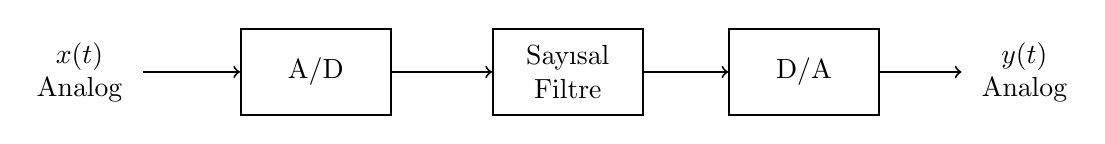
\begin{tikzpicture}[line width=0.7pt, box/.style={draw, minimum width=1.9cm, minimum height=1.1cm, align=center}]
  \node[box] (ad) at (0,0) {A/D};
  \node[box] (sf) at (3.2,0) {Sayısal\\Filtre};
  \node[box] (da) at (6.2,0) {D/A};
  \node[align=center] at (-3.0,0) {$x(t)$\\ Analog};
  \node[align=center] at (9.0,0) {$y(t)$\\ Analog};
  \draw[->] (-2.2,0) -- (ad.west);
  \draw[->] (ad.east) -- (sf.west);
  \draw[->] (sf.east) -- (da.west);
  \draw[->] (da.east) -- (8.2,0);
\end{tikzpicture}
\end{center}

\sayfa{5}
\section{Bir haberleşme kanalında işaret Bozulması}
\begin{itemize}
\item Lineer Bozulma\\(Lineer Distortion)
\end{itemize}
kanal ideal $\Rightarrow$ Bozulmasız (Distortionless)
\[
\begin{aligned}|H(f)|&=|k|\\\theta_h(f)&=-2\pi ft_d\end{aligned}\quad\Rightarrow\quad\begin{array}{l}\text{Biri sağlanmıyorsa kanal}\\\text{bozulmalı (with distortion)}\end{array}
\]
kanal bozulmalı ise $x(t)$ zamanda yayılır (time dispersion)

\begin{ornek}
(Lathi)
\end{ornek}
\[
H(f)=\begin{cases}\bigl(1+k\cos(2\pi fT)\bigr)\,e^{-j2\pi ft_d}, & |f|<B\\[2pt] 0, & \text{Else}\end{cases}
\]
\begin{center}
\begin{tikzpicture}[line width=0.7pt]
  \draw[->] (-2.6,0) -- (2.8,0) node[right] {$f$};
  \draw[->] (0,-0.1) -- (0,1.7) node[right] {$|H(f)|$};
  \draw[domain=-1.7:1.7,samples=40,smooth,variable=\x] plot ({\x},{0.95+0.25*cos(\x*52.94)});
  \draw[dashed] (-1.7,-0.3) -- (-1.7,0.95);
  \draw[dashed] (1.7,-0.3) -- (1.7,0.95);
  \node[below] at (-1.7,-0.3) {$-B$};
  \node[below] at (1.7,-0.3) {$B$};
  \draw[kirmizikalem,thick] (-1.5,0.95) -- (1.5,-0.95);
  \node[kirmizikalem,right] at (1.5,-0.95) {$-2\pi ft_d$};
\end{tikzpicture}
\end{center}
A LPF transfer function is given in the figure. A pulse $x(t)$ band-limited to $B$ Hz is applied at the input of this filter. Find the output $y(t)$

\begin{center}
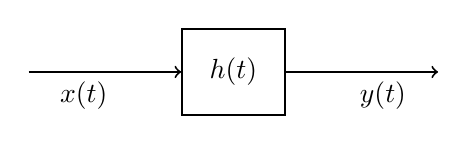
\begin{tikzpicture}[line width=0.7pt]
  \node[draw,minimum width=1.3cm,minimum height=1.1cm] (h) at (0,0) {$h(t)$};
  \draw[->] (-2.6,0) -- (h.west);
  \draw[->] (h.east) -- (2.6,0);
  \node[below] at (-1.9,0) {$x(t)$};
  \node[below] at (1.9,0) {$y(t)$};
\end{tikzpicture}
\end{center}
\begin{align*}
Y(f)&=X(f)H(f)=X(f)\Bigl[1+k\underbrace{\cos(2\pi fT)}_{\textcolor{kirmizikalem}{\frac12\left[e^{j2\pi fT}+e^{-j2\pi fT}\right]}}\Bigr]e^{-j2\pi ft_d}\\
Y(f)&=X(f)\,e^{-j2\pi ft_d}+k\,X(f)\cos(2\pi fT)\,e^{-j2\pi ft_d}
\end{align*}

\sayfa{6}
\noindent $\updownarrow\ F^{-1}$
\[
y(t)=x(t-t_d)+\frac{k}{2}\bigl[x(t+T-t_d)+x(t-T-t_d)\bigr]
\]
\[
x(t)+\frac{k}{2}\bigl[x(t+T)+x(t-T)\bigr]\ \xrightarrow{\,t_d\ \text{sabit}\,}
\]

\begin{ornek}
e.g
\begin{center}
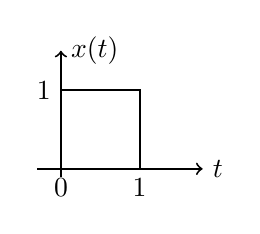
\begin{tikzpicture}[line width=0.7pt]
  \draw[->] (-0.3,0) -- (1.8,0) node[right] {$t$};
  \draw[->] (0,-0.1) -- (0,1.5) node[right] {$x(t)$};
  \draw (0,1) -- (1,1) -- (1,0);
  \node[left] at (0,1) {$1$};
  \node[below] at (0,0) {$0$};
  \node[below] at (1,0) {$1$};
\end{tikzpicture}
\end{center}
$k=1,\ T=0{,}5,\ t_d=2$
\end{ornek}

Burada \okunamadi{yankılık} var //

\begin{center}
\begin{tikzpicture}[line width=0.7pt, x=2cm, y=1.6cm]
  \draw[->] (-1.1,0) -- (2.2,0);
  \draw[->] (0,0) -- (0,1.6);
  \draw (0,0) -- (0,1) -- (1,1) -- (1,0);
  \node[above right] at (1,1) {$x(t)$};
  \draw[kirmizikalem!60] (-0.5,0) -- (-0.5,0.5) -- (0.5,0.5) -- (0.5,0);
  \draw[kirmizikalem] (0.5,0) -- (0.5,0.5) -- (1.5,0.5) -- (1.5,0);
  \node[below,font=\scriptsize] at (-0.5,0) {$-0{,}5$};
  \node[below,font=\scriptsize] at (0,0) {$0$};
  \node[below,font=\scriptsize] at (0.5,0) {$0{,}5$};
  \node[below,font=\scriptsize] at (1,0) {$1$};
  \node[below,font=\scriptsize] at (1.5,0) {$1{,}5$};
\end{tikzpicture}
\end{center}

\begin{center}
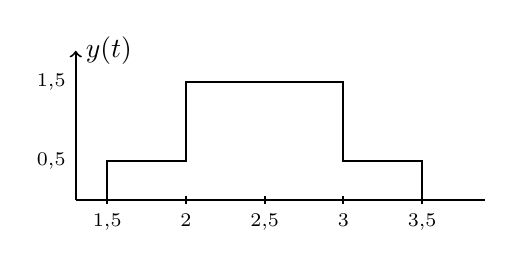
\begin{tikzpicture}[line width=0.7pt, x=2cm, y=1cm]
  \draw (1.3,0) -- (3.9,0);
  \draw[->] (1.3,0) -- (1.3,1.9) node[right] {$y(t)$};
  \draw (1.5,0) -- (1.5,0.5) -- (2,0.5) -- (2,1.5) -- (3,1.5) -- (3,0.5) -- (3.5,0.5) -- (3.5,0);
  \foreach \xa/\xl in {1.5/1{,}5, 2/2, 2.5/2{,}5, 3/3, 3.5/3{,}5} {\draw (\xa,0.05) -- (\xa,-0.05); \node[below,font=\scriptsize] at (\xa,-0.05) {$\xl$};}
  \node[left,font=\scriptsize] at (1.3,1.5) {$1{,}5$};
  \node[left,font=\scriptsize] at (1.3,0.5) {$0{,}5$};
\end{tikzpicture}
\end{center}

\begin{ornek}
eg \quad \textcolor{kirmizikalem}{$k=1,\ T=1{,}5,\ t_d=2$}
\begin{center}
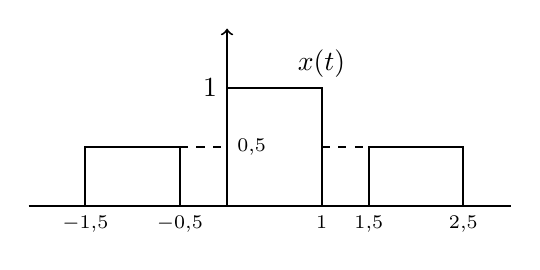
\begin{tikzpicture}[line width=0.7pt, x=1.2cm, y=1.5cm]
  \draw (-2.1,0) -- (3.0,0);
  \draw[->] (0,0) -- (0,1.5);
  \draw (0,0) -- (0,1) -- (1,1) -- (1,0);
  \draw (-1.5,0) -- (-1.5,0.5) -- (-0.5,0.5) -- (-0.5,0);
  \draw (1.5,0) -- (1.5,0.5) -- (2.5,0.5) -- (2.5,0);
  \draw[dashed] (-0.5,0.5) -- (0,0.5);
  \draw[dashed] (1,0.5) -- (1.5,0.5);
  \node[above] at (1,1) {$x(t)$};
  \node[left] at (0,1) {$1$};
  \node[right,font=\scriptsize] at (0,0.5) {$0{,}5$};
  \foreach \xa/\xl in {-1.5/-1{,}5, -0.5/-0{,}5, 1/1, 1.5/1{,}5, 2.5/2{,}5} {\node[below,font=\scriptsize] at (\xa,0) {$\xl$};}
\end{tikzpicture}
\end{center}
\end{ornek}

\sayfa{7}
\begin{itemize}
\item Linear olmayan bozulma\\(Non linear distortion)
\end{itemize}
\begin{center}
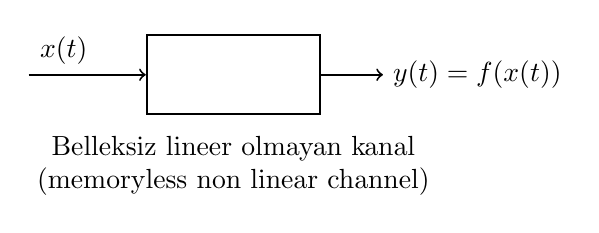
\begin{tikzpicture}[line width=0.7pt]
  \node[draw,minimum width=2.2cm,minimum height=1cm] (b) at (0,0) {};
  \draw[->] (-2.6,0) -- (b.west) node[pos=0.3,above] {$x(t)$};
  \draw[->] (b.east) -- (1.9,0) node[right] {$y(t)=f(x(t))$};
  \node[below,align=center] at (0,-0.65) {Belleksiz lineer olmayan kanal\\(memoryless non linear channel)};
\end{tikzpicture}
\end{center}
Maclaurin serisine açılırsa
\[
y(t)=f(x(t))=a_0+a_1x(t)+a_2x^2(t)+a_3x^3(t)+\cdots+a_kx^k(t)
\]
\[
\mathrm{BG}\{x(t)\}=B\qquad\qquad\mathrm{BG}\{x^k(t)\}=k\cdot B\ \mathrm{Hz}
\]
$\Rightarrow$ Frekansta yayılma\\(spectral dispersion)

\begin{ornek}
(Lathi)
\end{ornek}
\begin{center}
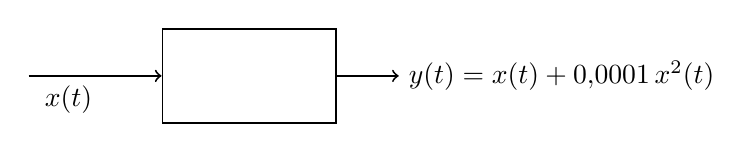
\begin{tikzpicture}[line width=0.7pt]
  \node[draw,minimum width=2.2cm,minimum height=1.2cm] (b) at (0,0) {};
  \draw[->] (-2.8,0) -- (b.west) node[pos=0.3,below] {$x(t)$};
  \draw[->] (b.east) -- (1.9,0) node[right] {$y(t)=x(t)+0{,}0001\,x^2(t)$};
\end{tikzpicture}
\end{center}
\begin{align*}
x(t)&=2000\,\mathrm{sinc}(2000t)\\
y(t)&=\ ?\qquad Y(f)=\ ?\qquad \mathrm{BW}\{y(t)\}=\ ?
\end{align*}
Can the signal $x(t)$ be recovered without distortion from the output $y(t)$?
\begin{align*}
A\tau\,\mathrm{sinc}(t\tau)&\overset{F}{\longleftrightarrow}A\,\Pi\!\left(\frac{f}{\tau}\right)\\
\underbrace{2000}_{\tau}\,\mathrm{sinc}(\underbrace{2000}_{\tau}\,t)&\overset{F}{\longleftrightarrow}X(f)=\Pi\!\left(\frac{f}{2000}\right)
\end{align*}
\begin{align*}
y(t)&=x(t)+0{,}0001\,x^2(t)\\
&=x(t)+400\,\mathrm{sinc}^2(2000t)
\end{align*}
\[
A\tau\,\mathrm{sinc}^2(t\tau)\overset{F}{\longleftrightarrow}A\,\Lambda\!\left(\frac{f}{\tau}\right)
\]

\sayfa{8}
\[
400\,\mathrm{sinc}^2(2000t)\overset{F}{\longleftrightarrow}0{,}2\,\Lambda\!\left(\frac{f}{2000}\right)
\]
\okunamadi{kırmızı not: $A=400/2000$}

\begin{align*}
y(t)&=2000\,\mathrm{sinc}(2000t)+400\,\mathrm{sinc}^2(2000t)\\
Y(f)&=\Pi\!\left(\frac{f}{2000}\right)+0{,}2\,\Lambda\!\left(\frac{f}{2000}\right)\ \checkmark
\end{align*}
\begin{center}
\begin{tikzpicture}[line width=0.7pt, x=1.5cm, y=1.5cm]
  \draw[->] (-2.5,0) -- (2.6,0) node[right] {$f$};
  \draw[->] (0,0) -- (0,1.5) node[above right] {$Y(f)$};
  \draw[kirmizikalem!55] (-2,0) -- (0,0.2) -- (2,0);
  \draw[kirmizikalem,thick] (-2,0) -- (-1,0.1) -- (-1,1.1) -- (0,1.2) -- (1,1.1) -- (1,0.1) -- (2,0);
  \node[font=\scriptsize,above] at (0,0.2) {$0{,}2$};
  \node[font=\scriptsize,above right] at (0,1.2) {$1{,}2$};
  \node[font=\scriptsize,left] at (-1,1.1) {$1$};
  \draw[->,kirmizikalem] (1.05,1.12) -- (1.4,1.12) node[right] {$Y(f)$};
  \node[below,font=\scriptsize] at (-2,0) {$-2000$};
  \node[below,font=\scriptsize] at (-1,0) {$-1000$};
  \node[below,font=\scriptsize] at (1,0) {$1000$};
  \node[below,font=\scriptsize] at (2,0) {$2000$};
\end{tikzpicture}
\end{center}
\[
\mathrm{BW}\{y(t)\}=2000\ \mathrm{Hz}
\]
\begin{center}
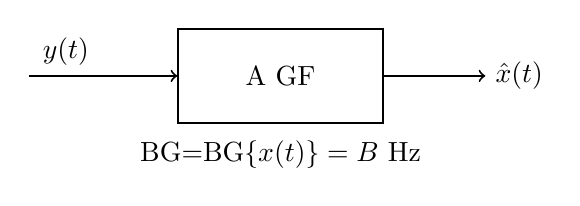
\begin{tikzpicture}[line width=0.7pt]
  \node[draw,minimum width=2.6cm,minimum height=1.2cm] (b) at (0,0) {A GF};
  \draw[->] (-3.2,0) -- (b.west) node[pos=0.25,above] {$y(t)$};
  \draw[->] (b.east) -- (2.6,0) node[right] {$\hat x(t)$};
  \node[below] at (0,-0.7) {BG$=$BG$\{x(t)\}=B$ Hz};
\end{tikzpicture}
\end{center}
\begin{center}
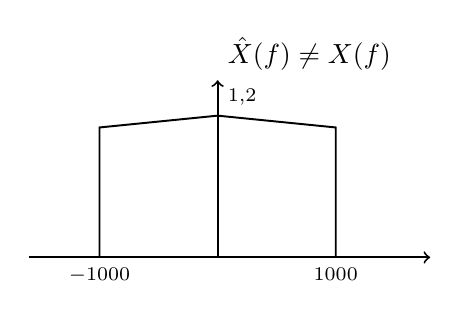
\begin{tikzpicture}[line width=0.7pt, x=1.5cm, y=1.5cm]
  \draw[->] (-1.6,0) -- (1.8,0);
  \draw[->] (0,0) -- (0,1.5) node[above right] {$\hat X(f)\neq X(f)$};
  \draw (-1,0) -- (-1,1.1) -- (0,1.2) -- (1,1.1) -- (1,0);
  \node[font=\scriptsize,above right] at (0,1.2) {$1{,}2$};
  \node[below,font=\scriptsize] at (-1,0) {$-1000$};
  \node[below,font=\scriptsize] at (1,0) {$1000$};
\end{tikzpicture}
\end{center}

Bozulma
\begin{itemize}
\item Lineer bozulma $\rightarrow$ zamanda yayılma $\rightarrow$ TDM'de karışım (interference)
\item Lineer olmayan bozulma $\rightarrow$ Frekansta yayılma $\rightarrow$ FDM'de karışım
\item[\textcolor{kirmizikalem}{$\star$}] Çok yollu bozulma (multipath distortion)
\end{itemize}

\section{Modülasyon (Modulation)}
Temel band işareti (Base band signal) $\rightarrow$ Baseband comm.\\
Temel bant haberleşmeyi (dijitalde yapılır)
\[
\left.\begin{array}{l}\text{Voice(ses)}:\ 0\text{-}4\,\mathrm{kHz}\\ \text{Video(görüntü)}:\ 0\text{-}5/6\,\mathrm{MHz}\ \text{(siyah-beyaz)}\end{array}\right\}\ \begin{array}{l}\text{Baseband analog signals}\\ \equiv\ \text{message signals}\end{array}
\]

\sayfa{9}
Modülasyon $\rightarrow$ Carrier communication\\
(Taşıyıcı haberleşme)

Alçak geçiren veya t.b. taki işaretin bg. hale geçirmektir.
\[
\mathrm{BG}\{m(t)\}=B,\quad M(f)=0,\quad |f|>B\ \Rightarrow\ \begin{array}{l}\text{Temel band}\\\text{işareti}\\\text{(Low pass signal)}\end{array}
\]

Taşıyıcı işaret (Carrier signal)
\[
c(t)=\underbrace{A_c}_{\substack{\text{Genlik}\\\text{(Amplitude)}}}\cos\Bigl(2\pi\underbrace{f_c}_{\substack{\text{Frekans}\\\text{(Freq)}}}t+\underbrace{\theta_c}_{\substack{\text{Faz}\\\text{(phase)}}}\Bigr)
\]
(Frekans ve Faz) $\rightarrow$ Açı modülasyonu

\section{Modülasyonun Sebepleri}
\begin{enumerate}[label=\arabic*)]
\item Frekans bölmeli çoklama (FDM) yapmak için\\
(Frequency Division multiplexing (FDM))\\
BTK haberleşme bandını söylüyor
\item Verici alıcı yapısını basitleştirmek için.\\
Dalga boyu küçülür
\[
\underset{\text{length of antenna}}{l}=\text{Anten boyu}\propto\frac{\lambda}{4}\ \rightarrow\ \text{Dalga boyu (wavelength)}
\]
\end{enumerate}
\[
\text{Ses BG}\approx3\,\mathrm{kHz}\qquad\qquad c=f\cdot\lambda\ \Rightarrow\ \lambda=\frac{c}{f}
\]
\[
=\frac{3\cdot10^8\ \mathrm{m/sn}}{3\cdot10^3\underbrace{\ \mathrm{Hz}}_{1/\mathrm{sn}}}
\]

\sayfa{10}
\[
=10^5\ \mathrm{m}=100\ \mathrm{km}\ \rightarrow\ l\approx\frac{\lambda}{4}=25\ \mathrm{km}
\]

Genlik modülasyonu (\okunamadi{yaptık}) : $f=1\,\mathrm{MHz}$
\[
\lambda=\frac{3\cdot10^8\ \mathrm{m/sn}}{10^6\ \mathrm{Hz}}=300\ \mathrm{m}\ \rightarrow\ l\approx\frac{\lambda}{4}=75\ \mathrm{m}
\]

\begin{enumerate}[label=\arabic*),start=3]
\item Mesaj işaretinin band genişliğini arttırarak gürültü ve karışımı bastırma özelliğini arttırmak için\\
(noise and interference immunity)\\
$\rightarrow$ Açı modülasyonu
\end{enumerate}

\end{document}
